\chapter{Analysis}
\label{chap:analysis}

In order to determine the feasibility of the proposed VFS, it is crucial to analyse existing alternatives.
In this chapter, we will delve into a detailed examination of various alternative solutions, highlighting their drawbacks and limitations.
Additionally, we will explore the essential libraries and tools required for the successful implementation of the proposed solution.
By thoroughly analyzing existing alternatives and exploring necessary components, we can better determine the viability of the proposed VFS\@.


\section{Analysis of Alternatives}\label{sec:alternatives}

The proposed solution presents a unique approach, as there is currently no existing virtual file system specifically designed to layer additional features atop pre-existing file systems.
Nevertheless, FUSE, the very library which was employed in developing this VFS, could be viewed as its competition, given that it can be utilized to enhance existing file systems with added features.
On the contrary, FUSE demands considerable effort to build a custom file system from scratch, and even if a developer undertakes the challenge, they would essentially be replicating a simplified version of this thesis' objective.

However, using VFS is not the only way to achieve the desired functionality of adding features, and in order to judge the potential benefits of our VFS, it is essential to individually examine alternative solutions that simply provide custom features on top of existing file systems.
This section will analyse existing non-virtual and virtual file systems with versioning and encryption features, as well as higher-level applications offering similar functionality.

Let us start with versioning; non-virtual versioning file systems is a well-documented concept, and there are several implementations available.
Notable non-virtual versioning file systems include OpenVMS, a versioning file system from Digital Equipment Corporation that automatically creates new instances of files with version numbers appended, and NILFS, a Linux-based log-structured file system that supports versioning and continuous snapshotting of the entire file system.
And even though these solutions would be viable options, they are not what someone might consider user-friendly.
They also offer limited configurability and extensibility, which is a significant drawback for a user who wants to customize the versioning process.

Still, several virtual file systems with versioning capabilities have been developed:

\begin{itemize}
    \item User space file systems implemented with FUSE:
    \begin{itemize}
        \item A simple versioning file system for Linux using FUSE\cite{simple_vfs}, written in Go.
        \item Wayback: A User-level Versioning File System for Linux\cite{wayback_vfs}, developed in Perl for the USENIX 2004 Annual Technical Conference using an older version of FUSE\@.
    \end{itemize}
    \item Copy-on-Write Version Support for VFS under Linux by Stephan Müller and Sven Widmer\cite{vvfs}, implemented as a kernel patch.
    \item A versioning virtual filesystem by Steve Huntley\cite{huntley_vvfs}, written in Tcl.
    However, this solution primarily serves as a language demonstration rather than a practical implementation.
\end{itemize}

These existing solutions are also not without various constraints, such as being platform-specific (mainly Linux-only) or discontinued.

The third option for versioning is to use higher-level applications.
These applications usually offer a wide range of features while still allowing extendability.
Some of the most popular applications include Git, Subversion, Time Machine, and Dropbox.
And to be honest, using these applications would be a practical solution, as they are well-maintained and offer a wide range of features.

Regarding encryption, while such focused VFSs are basically nonexistent, there are several non-virtual file systems that offer encryption capabilities, such as the EFS which provides cryptographic protection of individual files on NTFS file system volumes using a public-key system.
And surely enough, such solutions are viable options, but they from my personal experience lack the configurability and flexibility that a virtual file system can provide, and once more the extensibility is limited.
For instance, as a dual-boot user, if I would like to have my files encrypted on the common partition, it would be not possible or at least very difficult to achieve with existing solutions.

Moving back to the VFS domain, the closest example to the desired functionality is rvault\cite{rvault}, which focuses on encrypting small files (passwords, keys, and secrets) and makes them accessible through one-time password authentication.
However, this does differ from the intended functionality of the proposed VFS and could not be considered as an alternative, rather it may serve as a source of inspiration.
Again, the competition is mainly higher-level applications, such as Folder Lock, Gpg, or Encrypto.

\subsection{Drawbacks of higher-level applications}\label{subsec:drawbacks-of-higher-level-applications}

Since we now established that the main competition is higher-level applications, let us examine why developing proposed VFS is still a reasonable idea even though one might label it as ``overkill''.
While we are not saying that higher-level applications are not a viable option, they are not meant for the same user base.
Depending on specific solution, negative aspects could include problematic layering of additional features, limited multi-platform support and leaking implementation details to the user.
And even more importantly, users are limited to using that particular application, while with VFS they can use any application they want.
Yet, for the usage of VFS to be convenient, the user's application of choice would need to be slightly modified.

On that note, it is also worth noting that some operating systems, specifically macOS, provide built-in support for versioning and limited encryption features.
For example, macOS's Time Machine offers versioning the way that it is possible to revert to previous versions of files or restore deleted data.
However, these features are not available on other platforms, and they may not provide the desired level of control over the process.

So, while there are several existing solutions that offer versioning and encryption features, they are usually platform-specific, lack the desired level of control or extensibility.
Additionally, there are no existing virtual file systems that provide the desired functionality.


\section{Necessary libraries}\label{sec:libs}

In the development of a virtual file system, there are two primary approaches to consider: writing kernel drivers or utilizing a user space library.
Writing kernel drivers offers low-level access to the operating system but requires extensive knowledge of the kernel and platform-specific implementations.
This method can be time-consuming, error-prone, and challenging to maintain.
Furthermore, this would result in limited extensibility, as the kernel driver would be responsible for all the functionality of the file system.
Not to mention the fact that kernel drivers are platform-specific, and they must be re-written for each platform.
However, despite the tedious process, it may result in a more efficient and robust solution.

An alternative to writing kernel drivers is using a user space file system library, such as FUSE\@.
This type of library allows developers to focus on the functionality and logic of their custom file system, rather than the intricate details of kernel programming.
This approach is more portable and easier to maintain, but it may not be as efficient as a kernel driver.
Nonetheless, the performance difference between the two approaches is negligible in most cases, and the benefits of using a user space library heavily outweigh the drawbacks in this particular scenario.

\subsection{FUSE}\label{subsec:fuse}

FUSE (named after Filesystem in Userspace) is an open-source software interface that allows developers to create custom file systems in user space without the need for kernel modifications.
It operates by providing a bridge between the kernel's VFS layer and user-space file system implementations.
The kernel communicates with the user-space file system using a well-defined API, allowing developers to create file systems without the need for kernel-level programming.
This abstraction greatly simplifies the development process and reduces the risks associated with kernel modifications.

FUSE has gained widespread adoption due to its ease of use and modularity.
Many popular file systems have been implemented using FUSE, such as SSHFS, GlusterFS, S3FS and NTFS-3G, among others.
These implementations demonstrate the versatility and robustness of the FUSE framework in handling a wide range of file system requirements.
Yet, FUSE is not without its limitations.
It is arguable whether it is the best choice for a C++ implementation, as it is written in C, but more on that in a later section~\ref{sec:fuse-in-cpp}.
Another complication is its portability.
Fortunately, even though FUSE was initially designed for Linux, variants are available for other platforms, ensuring cross-platform compatibility:

\begin{itemize}
    \item \textbf{Linux}: libfuse - The reference implementation of FUSE~\cite{libfuse}.
    \item \textbf{macOS}: FUSE for macOS - A macOS port of FUSE~\cite{osxfuse}.
    \item \textbf{Windows}: WinFsp - A Windows File System Proxy that provides FUSE-compatible functionality~\cite{winfsp}.
\end{itemize}

To develop a new file system using FUSE, a handler program connected to the provided libfuse library must be created.
The primary objective of this handler program is to define the file system's behavior in response to read, write, and stat requests.
Additionally, the handler program is responsible for mounting the new file system.
Upon mounting, the handler is registered with the kernel.
When a user initiates read, write, or stat requests for the newly mounted file system, the kernel forwards these I/O requests to the handler, which processes them accordingly.
The handler's response is then relayed back to the user by the kernel, ensuring a seamless interaction between the custom file system and the operating system.

The FUSE flow-chart diagram created by Wikipedia user named Sven\cite{fuse-diagram} depicted in Figure~\ref{fig:fuse-diagram} effectively illustrates the process involved in handling a command like `ls', from its initial submission to the virtual file system layer, through the FUSE kernel module, to a handler program in user space and back.

\begin{figure}[ht]
    \centering
    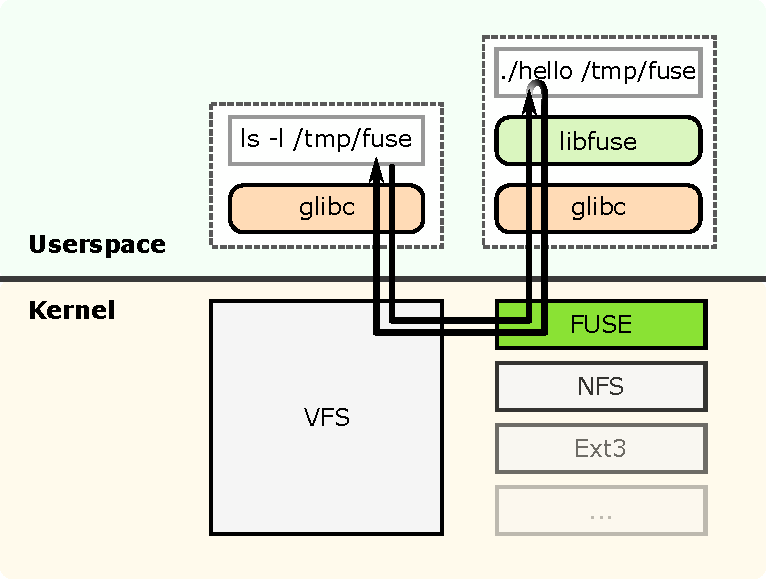
\includegraphics[width=0.8\linewidth]{img/fuse_diagram}
    \caption{FUSE flow-chart diagram}\label{fig:fuse-diagram}
\end{figure}

Considering the advantages of user space development and the availability of FUSE for multiple platforms, FUSE is my preferred choice for implementing the proposed VFS\@.
This approach enables the development of a cross-platform VFS with versioning and encryption capabilities while avoiding the complexity of kernel driver development.
Still, several other libraries will need to be employed to address various aspects of the project.

\subsection{Encryption}\label{subsec:encryption-analysis}

Initially, Crypto++\cite{crypto_pp} was considered for integration into the custom VFS, given its comprehensive open-source C++ class library covering a wide array of cryptographic schemes, such as encryption, hashing, and authentication algorithms.
Utilizing Crypto++ would provide file-level encryption, effectively safeguarding the security and privacy of the data stored within the VFS\@.

However, the implementation of Crypto++ led to various issues, primarily complicating the build process.
As a result, the decision was made to switch to libsodium\cite{libsodium}, which is a more user-friendly alternative.
It offers a robust selection of encryption, decryption, and cryptographic functions while maintaining a focus on simplicity and efficiency.
With that, the custom VFS can achieve the desired level of data protection without incurring the complexities associated with Crypto++.

\subsection{Testing}\label{subsec:gtest}

Google Test\cite{google_test}, commonly referred to as gtest, is a widely-used C++ testing framework developed by Google.
This library enables testing of individual components and the overall functionality of the custom VFS\@.
By employing gtest, the quality, reliability, and performance of the custom VFS can be evaluated, guaranteeing that it fulfills the requirements and expectations outlined in this thesis.

\subsection{Options parsing}\label{subsec:options-parsing}

The Boost Program Options library\cite{boost_program_options} is a C++ library used for option parsing, which makes it easy to parse command-line options and arguments.
This library has been utilized for the custom VFS to handle different command-line options effectively, including setting the mount point, enabling or disabling debugging mode, and so on.
Besides that, it was also used for the supporting tools.

The reason why this library was chosen in particular is because of its ease of use, popularity, and variety of features.

\subsection{Space for improvement}\label{subsec:libs-space-for-improvement}

While the libraries mentioned above have been used for the custom VFS, there are still some areas for improvement.
Mainly, some libraries could potentially be used instead of ``reinventing the wheel'' such as source code for handling of paths, configuration files, and logging.
But it is hard to say how severe this issue is, as all of these implementations are elementary and straightforward.
Furthermore, all of these implementations are written as such that they could be easily replaced with a library if needed.